\documentclass[a4paper,11pt,titlepage]{article}

%Εισαγωγή γλωσσικής υποστήριξης
%ελληνικό hyphenation

\usepackage[cm-default]{fontspec}
\usepackage{xunicode}
\usepackage{xltxtra}
\usepackage{xgreek}
\usepackage[colorlinks]{hyperref}
\usepackage{enumerate}
\usepackage{amsmath}
\usepackage{tikz}
\usepackage{float}
\usepackage{multirow}
%η γραμματοσειρά
%\setmainfont[Mapping=tex-text]{Times New Roman} %απλοποιημένο σε σχέση με το άρθρο
\setmainfont[Mapping=tex-text]{Linux Libertine} 
%page orientation
\usepackage{a4wide}
\voffset = -0.5in
\textheight = 664pt
\parindent = 0in
\newcommand{\degrees}{\ensuremath{^\circ}}

%Άλλα χρήσιμα πακέτα
\usepackage{graphicx} 	%εισαγωγή εικόνων jpg/png κλπ
\usepackage{listings}
\lstset
{
commentstyle=\textit,
captionpos=b,
breakatwhitespace=true,
showstringspaces=false,
breaklines=true,
keywordstyle=\color{black}\bfseries,
float=htb,
frame=single
}

%απενεργοποίηση του indent στις νέες παραγράφους
\parindent=0in

%macro που δίνει το μέγιστο επιτρεπτό μέγεθος σε μια εικόνα χωρίς να παραβιάζει τα όρια του LaTeX
\makeatletter
\def\maxwidth{
\ifdim\Gin@nat@width>\linewidth
\linewidth
\else
\Gin@nat@width
\fi
    }
\makeatother

\title{1η Άσκηση\\kn}
\author{Axil}
\date{\today}

\begin{document}

\pagestyle{headings}    %αρίθμηση στο πάνω μέρος της σελίδας

%\maketitle
\begin{titlepage}
\begin{center}

\includegraphics[width=50mm]{pyrforos.pdf}\\[0.5cm]
\textbf{\LARGE ΕΘΝΙΚΟ ΜΕΤΣΟΒΙΟ ΠΟΛΥΤΕΧΝΕΙΟ}\\
\textrm{\Large Σχολή Εφαρμοσμένων Μαθηματικών και Φυσικών Επιστημών}\\[2.0cm]
\Huge{Εργαστήριο Οπτοηλεκτρονικής}\\
\Large{\textit{7o εξάμηνο, ΣΕΜΦΕ}}\\[2.0cm]
\Large{\textit{\textbf{ Οπτικές ίνες}}}\\[5.0cm]
\normalsize
\begin{minipage}{0.49\textwidth}
\begin{flushleft}
\textbf{Πιπινέλλης Αχιλλέας}, 09103163
\end{flushleft}
\end{minipage}
\begin{minipage}{0.49\textwidth}
\begin{flushright}
\textbf{\textit{Η/Μ Παράδοσης:} 25 Ιανουαρίου 2012}
\end{flushright}
\end{minipage}
%\maketitle

\vfill
%bottom of the page
{Αθήνα, 2012}


\end{center}
\end{titlepage}

\section{Θεωρία}
\subsection{Τι είναι οι οπτικές ίνες;}
Οι οπτικές ίνες, είναι ειδικά νήματα που έχουν κατασκευαστεί από γυαλί ή πλαστικό με διάμετρο περίπου όσο μια ανθρώπινη τρίχα και μεταφέρουν το φως κατά μήκος τους. Με την βοήθεια των οπτικών ινών μπορούμε να “αναγκάσουμε” μια φωτεινή δέσμη να ακολουθήσει όποια διαδρομή επιθυμούμε. Θα μπορούσαμε να πούμε ότι, όπως με ένα εύκαμπτο λάστιχο ποτίσματος μπορούμε να οδηγήσουμε το νερό από την βρύση σε ένα σημείο του κήπου μας, έτσι και με τις οπτικές ίνες μπορούμε να “οδηγήσουμε” το φως από μια ακίνητη πηγή σε οποιοδήποτε σημείο θέλουμε. Γι’ αυτό λέμε ότι μια οπτική ίνα είναι ένας φωτοαγωγός ή φωτοοδήγος. Kάθε οπτική ίνα αποτελείται από τρία μέρη:
\begin{itemize}
\item Την κεντρική γυάλινη κυλινδρική ίνα, που ονομάζεται πυρήνας και είναι το τμήμα στο οποίο διαδίδεται το φως.
\item Την επικάλυψη (απλή ή πολλαπλή), που είναι ένας ομόκεντρος με τον πυρήνα κύλινδρος. Έχει μικρότερο δείκτη διάθλασης από τον πυρήνα, για να παθαίνει το φως συνεχείς ολικές ανακλάσεις. Η επικάλυψη αυτή ονομάζεται μανδύας
\item Το περίβλημα, που είναι ένα αδιαφανές πλαστικό.
\end{itemize}

\begin{figure} [hp!]
\centering
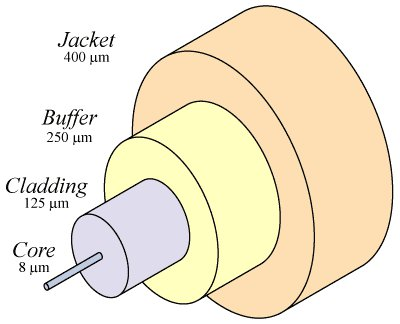
\includegraphics[width=60mm]{cable.jpg}
\caption{Οπτική ίνα}
\end{figure}
\newpage
\subsection{Τρόποι εκπομπής και μετάδοσης}
Η εκπομπή του οπτικού σήματος σε οπτική ίνα γίνεται από πηγή LED (Light Emmiting Diode) ή LASER (Light Amplification by Stimulated Emission of Radiation), και τα μήκη κύματος του φωτός, που η οπτική ίνα είναι σχεδιασμένη να μεταφέρει, ποικίλουν από 800nm μέχρι 1500nm. Οι οπτικές ίνες διαφοροποιούνται, κατ'αρχάς, από τον τρόπο μετάδοσης του σήματος σε αυτές. Η πρώτη βασική διάκριση είναι μεταξύ των πολυρυθμικών και μονορυθμικών οπτικών ινών.
\begin{itemize}

\item Πολυρυθμικές οπτικές ίνες (Multimode fiber optics)

Στις πολυρυθμικές ίνες διαδίδονται πολλοί ρυθμοί που αντιστοιχούν σε ακτίνες διαφορετικών διευθύνσεων και επομένως διαφορετικών γωνιών πρόσπτωσης. Το πλήθος των ρυθμών σε ίνες κλιμακωτού δείκτη διάθλασης προσδιορίζεται ως 
\begin{equation}
N = \frac{V^2}{2} , \; V = \frac{{\pi}d(NA)}{\lambda} \;
\end{equation}

Οι πολυρυθμικές οπτικές ίνες διακρίνονται σε δυο κατηγορίες: τις κλιμακωτού δείκτη διάθλασης (step index) και τις βαθμιαίου δείκτη διάθλασης (graded index).
\begin{itemize}

\item Οπτική ίνα διακριτού δείκτη (step index)
Στις ίνες αυτές συμβαίνει απότομη μεταβολή του δείκτη διάθλασης μεταξύ της κεντρικής ίνας και του υλικού επίστρωσης. Στην περίπτωση αυτή, η πορεία των ακτίνων εμφανίζεται στο Σχήμα 2.

\item Οπτική ίνα βαθμιαίου δείκτη (graded index)
Οι ίνες αυτές χαρακτηρίζονται από βαθμιαία μεταβολή του δείκτη διάθλασης του υλικού της κεντρικής ίνας. Συμβαίνει βαθμιαία μείωση όσο απομακρυνόμαστε από το κέντρο προς την εξωτερική επιφάνεια του γυαλιού. Η πορεία των ακτινών σε μια τέτοια ίνα είναι αυτή, που φαίνεται στο Σχήμα 3.
\end{itemize}

\item Μονορυθμικές οπτικές ίνες (single mode fiber optics)

Στις μονότροπες οπτικές ίνες η διάμετρος της κεντρικής ίνας είναι πολύ μικρή και πλησιάζει περίπου το επίπεδο του μήκους κύματος του εκπεμπόμενου σήματος. Στην περίπτωση αυτή, έχουμε έναν μόνο δυνατό τρόπο μετάδοσης του οπτικού σήματος, τον αξονικό. Η πορεία των ακτινών σε μια τέτοια οπτική ίνα φαίνεται στο Σχήμα 4. Η κεντρική ίνα στις μονότροπες οπτικές ίνες έχει διάμετρο από 5μm έως 10μm με συνηθέστερη τιμή τα 8,3 μm.
\end{itemize}
\newpage
\begin{figure} [H]
\centering
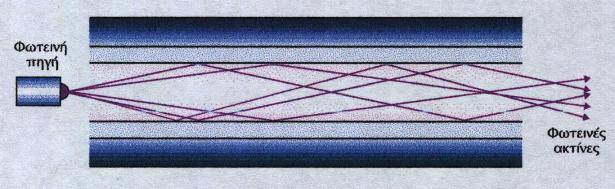
\includegraphics[width=100mm]{step_index.jpg}
\caption{Οπτική ίνα διακριτού δείκτη}
\end{figure}

\begin{figure} [H] 
\centering
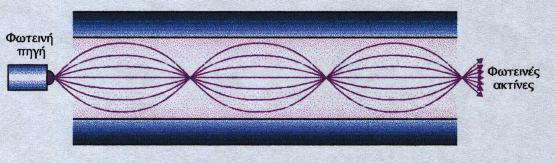
\includegraphics[width=100mm]{graded_index.jpg}
\caption{Οπτική ίνα βαθμιαίου δείκτη}
\end{figure}

\begin{figure} [H] 
\centering
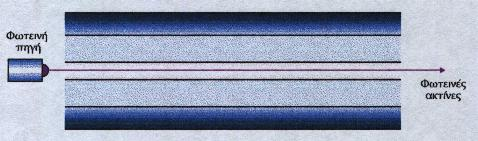
\includegraphics[width=100mm]{single_mode.jpg}
\caption{Μονορυθμική οπτική ίνα}
\end{figure}


\subsection{Φαινόμενα εξασθένισης σήματος}
Το φως κατά το “ταξίδι” του σε μια οπτική ίνα εξασθενεί. Αυτό συμβαίνει συνήθως για τους παρακάτω λόγους:
\begin{itemize}
\item Λόγω απορρόφησης, που οφείλεται στις ξένες προσμείξεις που υπάρχουν στο γυαλί 
\item Λόγω σκέδασης το φως διεισδύει στο μανδύα και διασκορπίζεται. Το φαινόμενο αυτό παρατηρείται εντονότερα, αν στην οπτική ίνα υπάρχουν συνδέσεις.
\item Λόγω κακής κατασκευής υπάρχουν στην διάμετρο του πυρήνα, για παράδειγμα, μικροδιακυμάνσεις.
\item Λόγω μεγάλης καμπής της οπτικής ίνας.
\end{itemize}

\newpage
\subsection{Πλεονεκτήματα/Μειονεκτήματα}

Οι οπτικές ίνες φαίνεται να είναι σήμερα η καλύτερη λύση στα μέσα μετάδοσης και αυτό γιατί τα πλεονεκτήματα, που παρουσιάζουν, σε σχέση με τα άλλα μέσα είναι ιδιαίτερα σημαντικά. Διαθέτουν πολύ μεγάλο εύρος ζώνης συχνοτήτων, με αποτέλεσμα να επιτυγχάνονται υψηλές ταχύτητες μετάδοσης (της τάξης των Gbps). Συνήθεις ταχύτητες μετάδοσης είναι αυτές των 2 και 10 Gbps, ενώ έχουν επίσης αναπτυχθεί συστήματα των 20,40 και 50 Gbps. Σε περίπτωση πολυπλεξίας με διαίρεση μήκους κύματος, οι ταχύτητες φθάνουν στα μερικά Tbps. Επίσης, δεν επηρεάζονται από ηλεκτρικά και μαγνητικά πεδία, με αποτέλεσμα να συνιστάται η χρήση τους σε βιομηχανικό περιβάλλον και σε χώρους με υψηλό θόρυβο. Η εξασθένηση των σημάτων είναι μικρότερη από ό,τι στα χάλκινα και ομοαξονικά καλώδια, με αποτέλεσμα οι αποστάσεις μεταξύ ενισχυτών ή άλλων ενεργών στοιχείων να κυμαίνονται από μερικά μέχρι και μερικές εκατοντάδες χιλιόμετρα, ανάλογα με τη τεχνική και το ρυθμό μετάδοσης. Η υποκλοπή ή η παρεμβολή πληροφορίας είναι πολύ δύσκολο να επιτευχθούν, με αποτέλεσμα οι οπτικές ίνες να συνιστούν πολύ ασφαλές μέσο μετάδοσης.
Επίσης, το βάρος και ο όγκος τους είναι σημαντικά μικρότερος από τα αντίστοιχα μεγέθη των άλλων αγωγών. Αξίζει να αναφέρουμε, ως παράδειγμα, ότι χάλκινο καλώδιο με 1000 ζεύγη και μήκος 500 μέτρων ζυγίζει περίπου 4000 κιλά, ενώ οπτική ίνα του ίδιου μήκους, που περιέχει τον ίδιο αριθμό καναλιών, ζυγίζει μόνο 45 κιλά.
\\
Επιπλέον, δεν είναι ευαίσθητες σε υγρό περιβάλλον, όπου τα χάλκινα καλώδια μπορεί να δημιουργήσουν βραχυκυκλώματα. Επειδή η οπτική ίνα δεν μεταφέρει ηλεκτρικό σήμα, προτιμάται σε περιοχές υψηλού κίνδυνου εκρήξεων από σπινθήρες (χώροι καυσίμων, εύφλεκτων αερίων κλπ.). Τα καλώδια οπτικών ινών παρουσιάζουν ίδιες μηχανικές ιδιότητες με τα ομοαξονικά, αλλά είναι ελαφρότερα σε βάρος, μικρότερα σε διάμετρο και οι αποστάσεις μεταξύ των επαναληπτών είναι μεγαλύτερες.
Ένα από τα βασικότερα μειονεκτήματα, που παρουσιάζουν οι οπτικές ίνες, είναι η δυσκολία υλοποίησης συνδέσεων, επειδή απαιτείται υψηλή προσαρμογή και ευθυγράμμιση της φωτεινής πηγής, για να μην υπάρχει διασπορά και να ελαχιστοποιηθούν οι απώλειες.
Όμως, η πρόοδος της τεχνολογίας, που έχει σημειωθεί τα τελευταία έτη στην περιοχή των οπτικών ινών, αντιμετώπισε με επιτυχία την παραπάνω δυσκολία, με αποτέλεσμα να είναι δυνατή η χρήση τους και για συνδέσεις σημείου προς πολλά σημεία. Παρ' όλα αυτά, η χρήση τους σε τέτοιες συνδέσεις δεν έχει ακόμη ευρέως εξαπλωθεί, ιδιαίτερα λόγω του αυξημένου κόστους, που παρουσιάζουν τέτοια συστήματα. 

\subsection{Πού τις χρησιμοποιούμε}

Οι οπτικές ίνες βρίσκουν πάρα πολλές εφαρμογές εκτός της πιο διαδεδομένης που αφορά στις τηλεπικοινωνίες. Οπτικές ίνες μεγάλης διαμέτρου και μικρής καθαρότητας (συνήθως πλαστικές) χρησιμοποιούνται στην κατασκευή φωτεινών επιγραφών, στην διακόσμηση και στο φωτισμό των πισίνων. Έτσι αποτρέπεται ο κίνδυνος ηλεκτροπληξίας. Δέσμη οπτικών ινών (με μια μόνο λάμπα) φωτίζει πολλές προθήκες καταστημάτων ή πολλούς πίνακες ζωγραφικής στις γκαλερί, ώστε να εξοικονομούμε ηλεκτρική ενέργεια. Με την βοήθεια των οπτικών ινών μπορούμε να παρατηρήσουμε αντικείμενα απρόσιτα σε άμεση παρατήρηση. Έτσι κατασκευάστηκε το ενδοσκόπιο, όργανο που χρησιμοποιείται στην Ιατρική, για να κάνει ορατές ορισμένες εσωτερικές περιοχές του σώματός μας. Παρόμοια συστήματα χρησιμοποιούνται από τους μηχανικούς για να εντοπίσουν βλάβες στο εσωτερικό των μηχανών. Επίσης οι οπτικές ίνες χρησιμοποιούνται σε σύγχρονα επιστημονικά όργανα ανίχνευσης παραμορφώσεων, πίεσης, θερμοκρασίας (ηφαιστείων και πυρηνικών αντιδραστήρων), καθώς και άλλων μεγεθών.
\newpage

\section{Πείραμα}

\subsection{Σύζευξη Οπτικής Ίνας - Δέσμης Laser}

Τα εξαρτήματα που χρησιμοποιήσαμε ήταν τα εξής;
\begin{itemize}
\item Laser He-Ne
\item Συζεύκτης laser-ίνας
\item Πολυρυθμική ίνα
\item Φωρατής
\end{itemize}

Αποδοτική ζεύξη επιτυγχάνεται μέσω ελέγχου της γωνίας μεταξύ δέσμης laser και φακού εστίασης. Ο συζέυκτης προσαρμόζεται στην έξοδο του laser. Aρχικά μετρήσαμε την ισχύ(y) της δέσμης του laser με το φωρατή, που έχει καμπύλη βαθμονόμησης η οποία δίνεται από την παρακάτω σχέση:
\\\\
\begin{equation}
y(mW) = 5 + 33*x(Volt)
\end{equation}
\\
Προσαρμόσαμε το συζευκτή στην έξοδο του laser και ρυθμίσαμε τη θέση του φακού εστίασης ως προς τη δέσμη μέχρι να κεντριστεί πάνω στον άξονα του laser. Συνδέσαμε την πολυρυθμική ίνα με το συζευκτή και ρυθμίσαμε τις βίδες, έτσι ώστε να συγκεντρώνεται όσο το δυνατόν περισσότερο φως στο κέντρο του φωτεινού ίχνους στην έξοδο της ίνας. Μετρήσαμε την ισχύ της δέσμης στην έξοδο της ίνας. Από την παρακάτω σχέση υπολογίζουμε την εξασθένιση της δέσμης (σε dB):
\\\\
\begin{equation}
IL=10 \log_{10} (P_{out}/P_{in})
\end{equation}
\\
Καταχωρήσαμε όλες τις μετρήσεις μας στον πίνακα 1. \\\\

\begin{table} [bph!]
\centering
\begin{tabular}{|c|c|c|c|}
\hline \rule[-2ex]{0pt}{5.5ex} Ένδειξη εξόδου ενεργόμετρου & Τάση (V) & Ισχύς (mW) & IL (dB) \\ 
\hline \rule[-2ex]{0pt}{5.5ex} Laser $(P_{in})$ & 0.553 & 23.249 & - \\
\hline \rule[-2ex]{0pt}{5.5ex} 1η οπτική ίνα $(P_{out})$ & 0.517 & 22.061 & -0.2278 \\ 
\hline 
\end{tabular} 
\caption{Αρχικές ενδείξεις}
\end{table} 

\newpage

\subsection{Προσδιορισμός αριθμητικού ανοίγματος οπτικής ίνας} %4.2

Σε αυτό το τμήμα της άσκησης θα προσδιορίσουμε το αριθμητικό άνοιγμα από τις διαστάσεις του φωτεινού ίχνους στην έξοδο της ίνας και από την απόσταση στην οποία θα απεικονίζουμε το φωτεινό ίχνος. Πέρα από τα εξαρτήματα που χρησιμοποιήσαμε στο προηγούμενο κομμάτι της άσκησης, θα χρησιμοποιήσουμε και μία οθόνη, ένα χάρακα και ένα χαρτί milimetre.\\
Αρχικά στερεώνουμε το χαρτί milimetre πάνω στην οθόνη απέναντι από το άκρο της ίνας, που είναι πάνω στο στήριγμα. Για 6 διαφορετικές θέσεις της οθόνης πάνω στον άξονα της οπτικής ίνας και της οθόνης από 3 έως 16 $cm$, μετρήσαμε τη διάμετρο $d$ της δέσμης πάνω στην οθόνη. Καταχωρήσαμε τα πειραματικά μας δεδομένα στον πίνακα 2. 
Από τον πίνακα 2 κάναμε το διάγραμμα 1, όπου δείχνει τη διάμετρο d σε σχέση με την απόσταση x.
Η γωνία του κώνου υποδοχής δίνεται από την παρακάτω σχέση:	
\begin{equation}
tanθ=\frac{d/2}{x}
\end{equation}
\\
Το αριθμητικό άνοιγμα της δέσμης δίνεται από τη σχέση:	
\begin{equation}
NA=sin\theta	
\end{equation}

\begin{table} [bph!]
\centering
\begin{tabular}{|c|c|c|c|c|}
\hline \rule[-2ex]{0pt}{5.5ex} $x (cm)$ 	& $d (cm)$ 	& $tan\theta$ 	& $\theta$ 	& $NA$ 		\\
\hline \rule[-2ex]{0pt}{5.5ex} 3.0 		& 2.4 		& 0.400 		& 21.80 	& 0.372 	\\
\hline \rule[-2ex]{0pt}{5.5ex} 5.0 		& 3.6 		& 0.360 		& 19.80 	& 0.339 	\\
\hline \rule[-2ex]{0pt}{5.5ex} 8.0 		& 5.0 		& 0.313 		& 17.38 	& 0.298 	\\
\hline \rule[-2ex]{0pt}{5.5ex} 10.0 	& 5.7 		& 0.285 		& 15.91 	& 0.274 	\\
\hline \rule[-2ex]{0pt}{5.5ex} 13.0 	& 6.4 		& 0.246 		& 13.82 	& 0.239 	\\
\hline \rule[-2ex]{0pt}{5.5ex} 16.0 	& 8.0 		& 0.250 		& 14.04 	& 0.243 	\\
\hline 
\end{tabular} 
\caption{Αριθμητικό άνοιγμα ίνας}
\end{table} 

Το αριθμητικό άνοιγμα του συστήματος laser-συζευκτής δίνεται από τη σχέση:	
\begin{equation}
NA_{δέσμης}=\frac{B.D.}{2f}
\end{equation}

όπου $B.D.=3mm$ , $f=1mm$ δηλαδή: $NA_{δέσμης} =1,5$.\\\\

Παρατηρούμε ότι το αριθμητικό άνοιγμα της δέσμης είναι πολύ μεγαλύτερο από το αριθμητικό άνοιγμα της ίνας. Αυτό οφείλεται στο γεγονός ότι εστιάσαμε τη δέσμη ώστε να διεγείρουμε τις αξονικές ακτίνες (και όχι τις περιφεριακές) με αποτέλεσμα να ελαττωθεί το αριθμητικό άνοιγμα.

\newpage

\subsection{Προσδιορισμός της Εξασθένησης Δέσμης κατά τη Σύζευξη 2 Οπτικών Ινών}%4.4

Η ζεύξη μεταξύ οπτικών ίνων εξαρτάται από 6 παράγοντες:
\begin{itemize}
\item Πλευρική απόκλιση 
\item Γωνιακή απόκλιση
\item Χωρισμός των άκρων
\item Κατεργασία των άκρων
\item Εσωτερικές απώλειες
\item Απώλειες Fresnel
\end{itemize}
Στο πείραμα μας θα χρησιμοποιήσουμε τα εξαρτήματα των προηγουμένων πειραμάτων καθώς και μία δεύτερη πολυρυθμική οπτική ίνα και τα εξαρτήματα για τη σύνδεση των 2 οπτικών ίνων. Έχουμε ήδη τη μέτρηση για την ισχύ στην έξοδο της πρώτης ίνας, έτσι αφού συνδέσαμε και τη δεύτερη ίνα πάνω στην πρώτη, μετρήσαμε την ισχύ της δέσμης έχοντας τις οπτικές ίνες χαλαρές. Στη συνέχεια μετρήσαμε την ισχύ της δέσμης, αφού τυλίξαμε τη  δεύτερη ίνα όσο πιο πολύ μπορούσαμε. Καταχωρήσαμε τις μετρήσεις μας στον πίνακα 3, μαζί με την υπολογισμένη απώλεια.

\begin{table} [bph!]
\centering
\begin{tabular}{|c|c|c|c|}
\hline \rule[-2ex]{0pt}{5.5ex} Ένδειξη εξόδου ενεργόμετρου & Τάση (V) & Ισχύς (mW) & IL (dB) \\ 
\hline \rule[-2ex]{0pt}{5.5ex} 1η οπτική ίνα & 0.517 $(P_{in})$  & 22.061 & - \\ 
\hline \rule[-2ex]{0pt}{5.5ex} 2η οπτική ίνα  & 0.500 & 21.500 $(P_{out})$ & -0.112 \\ 
\hline \rule[-2ex]{0pt}{5.5ex} 2η οπτική ίνα τυλιγμένη  & 0.365 & 17.045 $(P_{out2})$ & -1.120 \\ 
\hline 
\end{tabular} 
\caption{Σύζευξη 2 οπτικών ινών}
\end{table}


\subsection{Προσδιορισμός του Συντελεστή Εξασθένησης Οπτικής Ίνας}%4.5

Σε αυτή την άσκηση θα προσδιορίσουμε το συντελεστή εξασθένισης οπτικής ίνας χρησιμοποιώντας μία βίδα η οποία θα παρεμβάλεται στην πορεία της δέσμης.\\
Συνδέσαμε τη δεύτερη οπτική ίνα με το φωρατή, παρεμβάλοντας τον εξασθενητή μεταξύ των δύο ινών.  Αρχικά περιστρέφουμε τη βίδα κατά 90\degrees και μετράμε την ισχύ της δέσμης. Επαναλάβαμε για πέντε βήματα και καταγράψαμε τις μετρήσεις στον πίνακα 4. Παρατηρούμε πως καθώς περιστρέφεται η βίδα, εξασθενεί η δέσμη laser και αυτό φαίνεται από την αντίστοιχη πτώση της ισχύος της. \\
Η ισχύς της δέσμης σε $dB$ υπολογίζεται από τη σχέση:

\begin{equation}
dB=10\log{P_{out}}\\
\end{equation}
\\

και η εξασθένιση της δέσμης $P_{n}-P_{in}$ σε $dB$ αντίστοιχα από:

\begin{equation}
IL=10 \log_{10} (P_{n}/P_{in})
\end{equation}\\

όπου $n$ ο αριθμός των στροφών.

\newpage

\begin{table} [bph!]
\centering
\begin{tabular}{|c|c|c|c|c|}
\hline \rule[-2ex]{0pt}{5.5ex}	Στροφές (\degrees)	& Τάση του φωρατή $(V)$ 	& Ισχύς δέσμης $(mW)$ & 	Ισχύς δέσμης $(dB)$ & $IL	P_{n}-P_{in} (dB)$ 	\\ 
\hline \rule[-2ex]{0pt}{5.5ex} 1	(90\degrees)	&	0.324 	&	15.69	&	11.96	&	-1.48	\\ 
\hline \rule[-2ex]{0pt}{5.5ex} 2	(180\degrees)	&	0.315	&	15.40	&	11.88	&	-1.56	\\ 
\hline \rule[-2ex]{0pt}{5.5ex} 3 	(270\degrees)	&	0.260 	&	13.58	&	11.33	&	-2.11	\\ 
\hline \rule[-2ex]{0pt}{5.5ex} 4	(360\degrees)	&	0.253 	&	13.35	&	11.25	&	-2.18	\\ 
\hline \rule[-2ex]{0pt}{5.5ex} 5	(450\degrees)	&	0.233 	&	12.69	&	11.03	&	-2.40	\\
\hline \rule[-2ex]{0pt}{5.5ex} 6	(540\degrees)	&	0.200	&	11.60	&	10.64	&	-2.79	\\  
\hline 
\end{tabular} 
\caption{Εξασθένιση ισχύος οπτικών ινών}
\end{table}

Στο διάγραμμα 2 έχει σχεδιαστεί η εξασθένηση $P_n - P_{in}$ ως συνάρτηση του πλήθους στροφών της βίδας. Θεωρητικά ο αριθμός στροφών της βίδας που αντιστοιχεί σε εξασθένηση $3dB$ ($50\%$) παρατηρείται όταν η βίδα καλύπτει το ήμισυ της δέσμης. Η μετατόπιση της βίδας είναι $64mm$ ανά $360\degrees$. Ο αριθμός στροφών της βίδας που αντιστοιχεί σε εξασθένηση $3dB$ υπολογίζεται από τον τύπο:

\begin{equation}
n = \frac{BD}{2*0.64}
\end{equation}\\

και είναι ίσος με $2.34$, όπου $B.D.$ η διάμετρος της δέσμης η οποία μας δίνεται ίση με $3mm$.
Από το διάγραμμα υπολογίζουμε τον αριθμό στροφών της βίδας που αντιστοιχεί σε εξασθένηση \\ 
$3dB + I.L.$, δηλαδή $3.112$ $dB$ και το οποίο είναι περίπου 6,5 στροφές (~600\degrees). \\

Παρατηρούμε μια σημαντική διαφορά της θεωρητικής τιμής από την πειραματική. Αυτό μπορεί να οφείλεται στη μη ακριβή ρύθμιση της βίδας του εξασθενητή καθώς και από τον όχι και τόσο αποδοτικό τρόπο με τον οποίο μετρούσαμε την ένταση της δέσμης, καθώς το φως του υποβάθρου αλλοίωνε τα αποτελέσματά μας.
\newpage

\begin{figure} [H] 
\centering
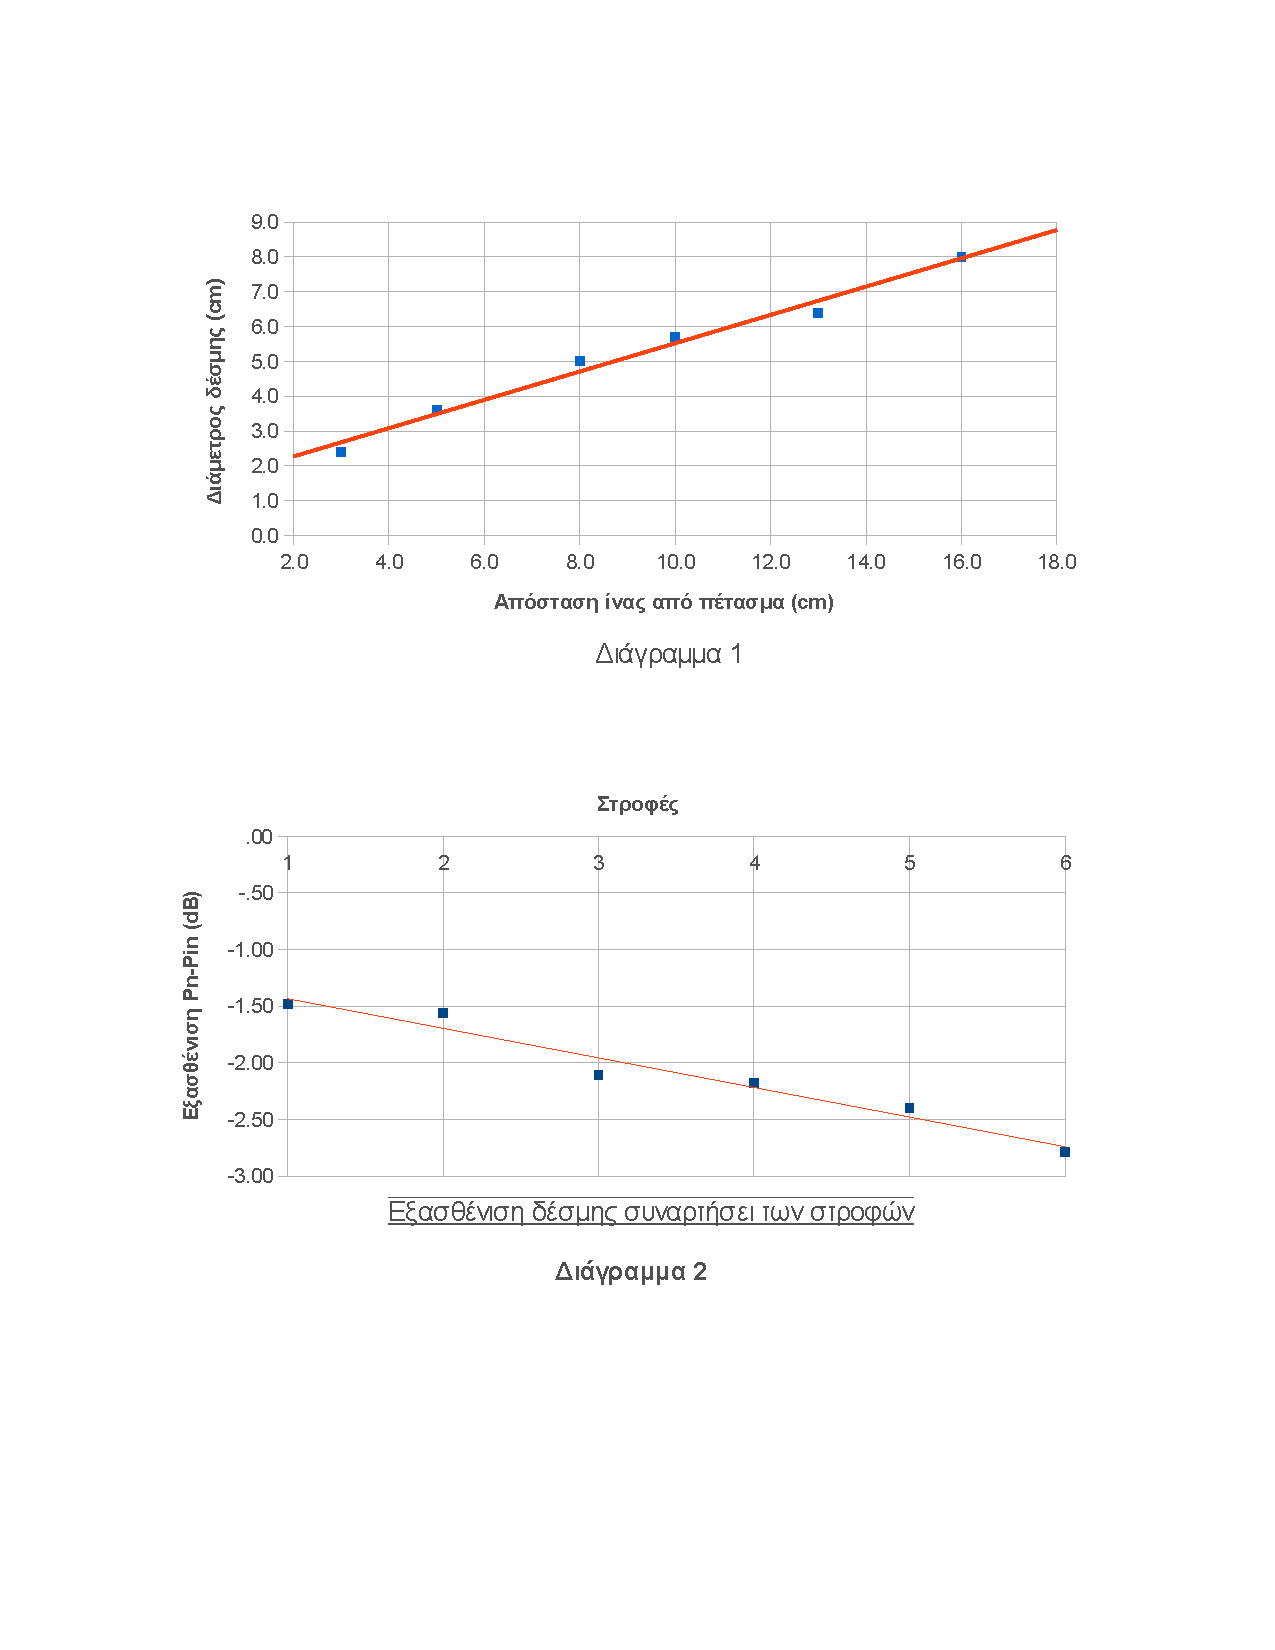
\includegraphics[width=\maxwidth]{graphs.pdf}
\end{figure}



%\begin{thebibliography}{9}

%\bibitem{internet articles}  $http://egnatia.ee.auth.gr/~aalexioy/fiber_op.htm http://3lyk-kalam.mes.sch.gr/opt_fiber_gr.htm http://el.science.wikia.com/wiki/Οπτική _Ίνα http://www.techteam.gr/wiki/Οπτικές _Ίνες$
%\bibitem{rp-photonics.com} Encyclopedia of Laser Physics and Technology, www.rp-photonics.com
%\bibitem{semfe} Εργαστηριακές Ασκήσεις Οπτοηλεκτρονικής - Φυσικής και τεχνολογίας των Lasers, ΕΜΠ ΣΕΜΦΕ Τομέας Φυσικής, Αθήνα 2005
%\bibitem{Young}  Hugh D. Young, Ηλεκτρομαγνητισμός - Οπτική - Σύγχρονη Φυσική, Εκδόσεις Παπαζήση, 8η έκδοση 1994 
%\bibitem{M.Young} Matt Young, Οπτική και Λέιζερ, Εκδόσεις ΕΜΠ, 2η έκδοση 2008 

%\end{thebibliography}

\end{document}
